\section{Porting Challenges}

Although the pre-Exascale machines gave the VTK-m development team good experience porting to different processor architectures, the design of the Exascale machines Frontier and Aurora introduced new technical challenges.
This section reports the most major modifications of VTK-m to make it feasible to run on the Exascale hardware.

\ken{
  Each subsection should be roughly 1/3 page.
  (1 + 1/3 page total.)
  The subsection should start with a paragraph defining the problem/motivation.
  The following paragraph should give an overview of the approach.
  The remaining paragraphs can go into technical challenges that were encountered and how they were addressed.
}

\subsection{Adopting Kokkos}

\assign{Sujin}

\begin{figure}[htb]
  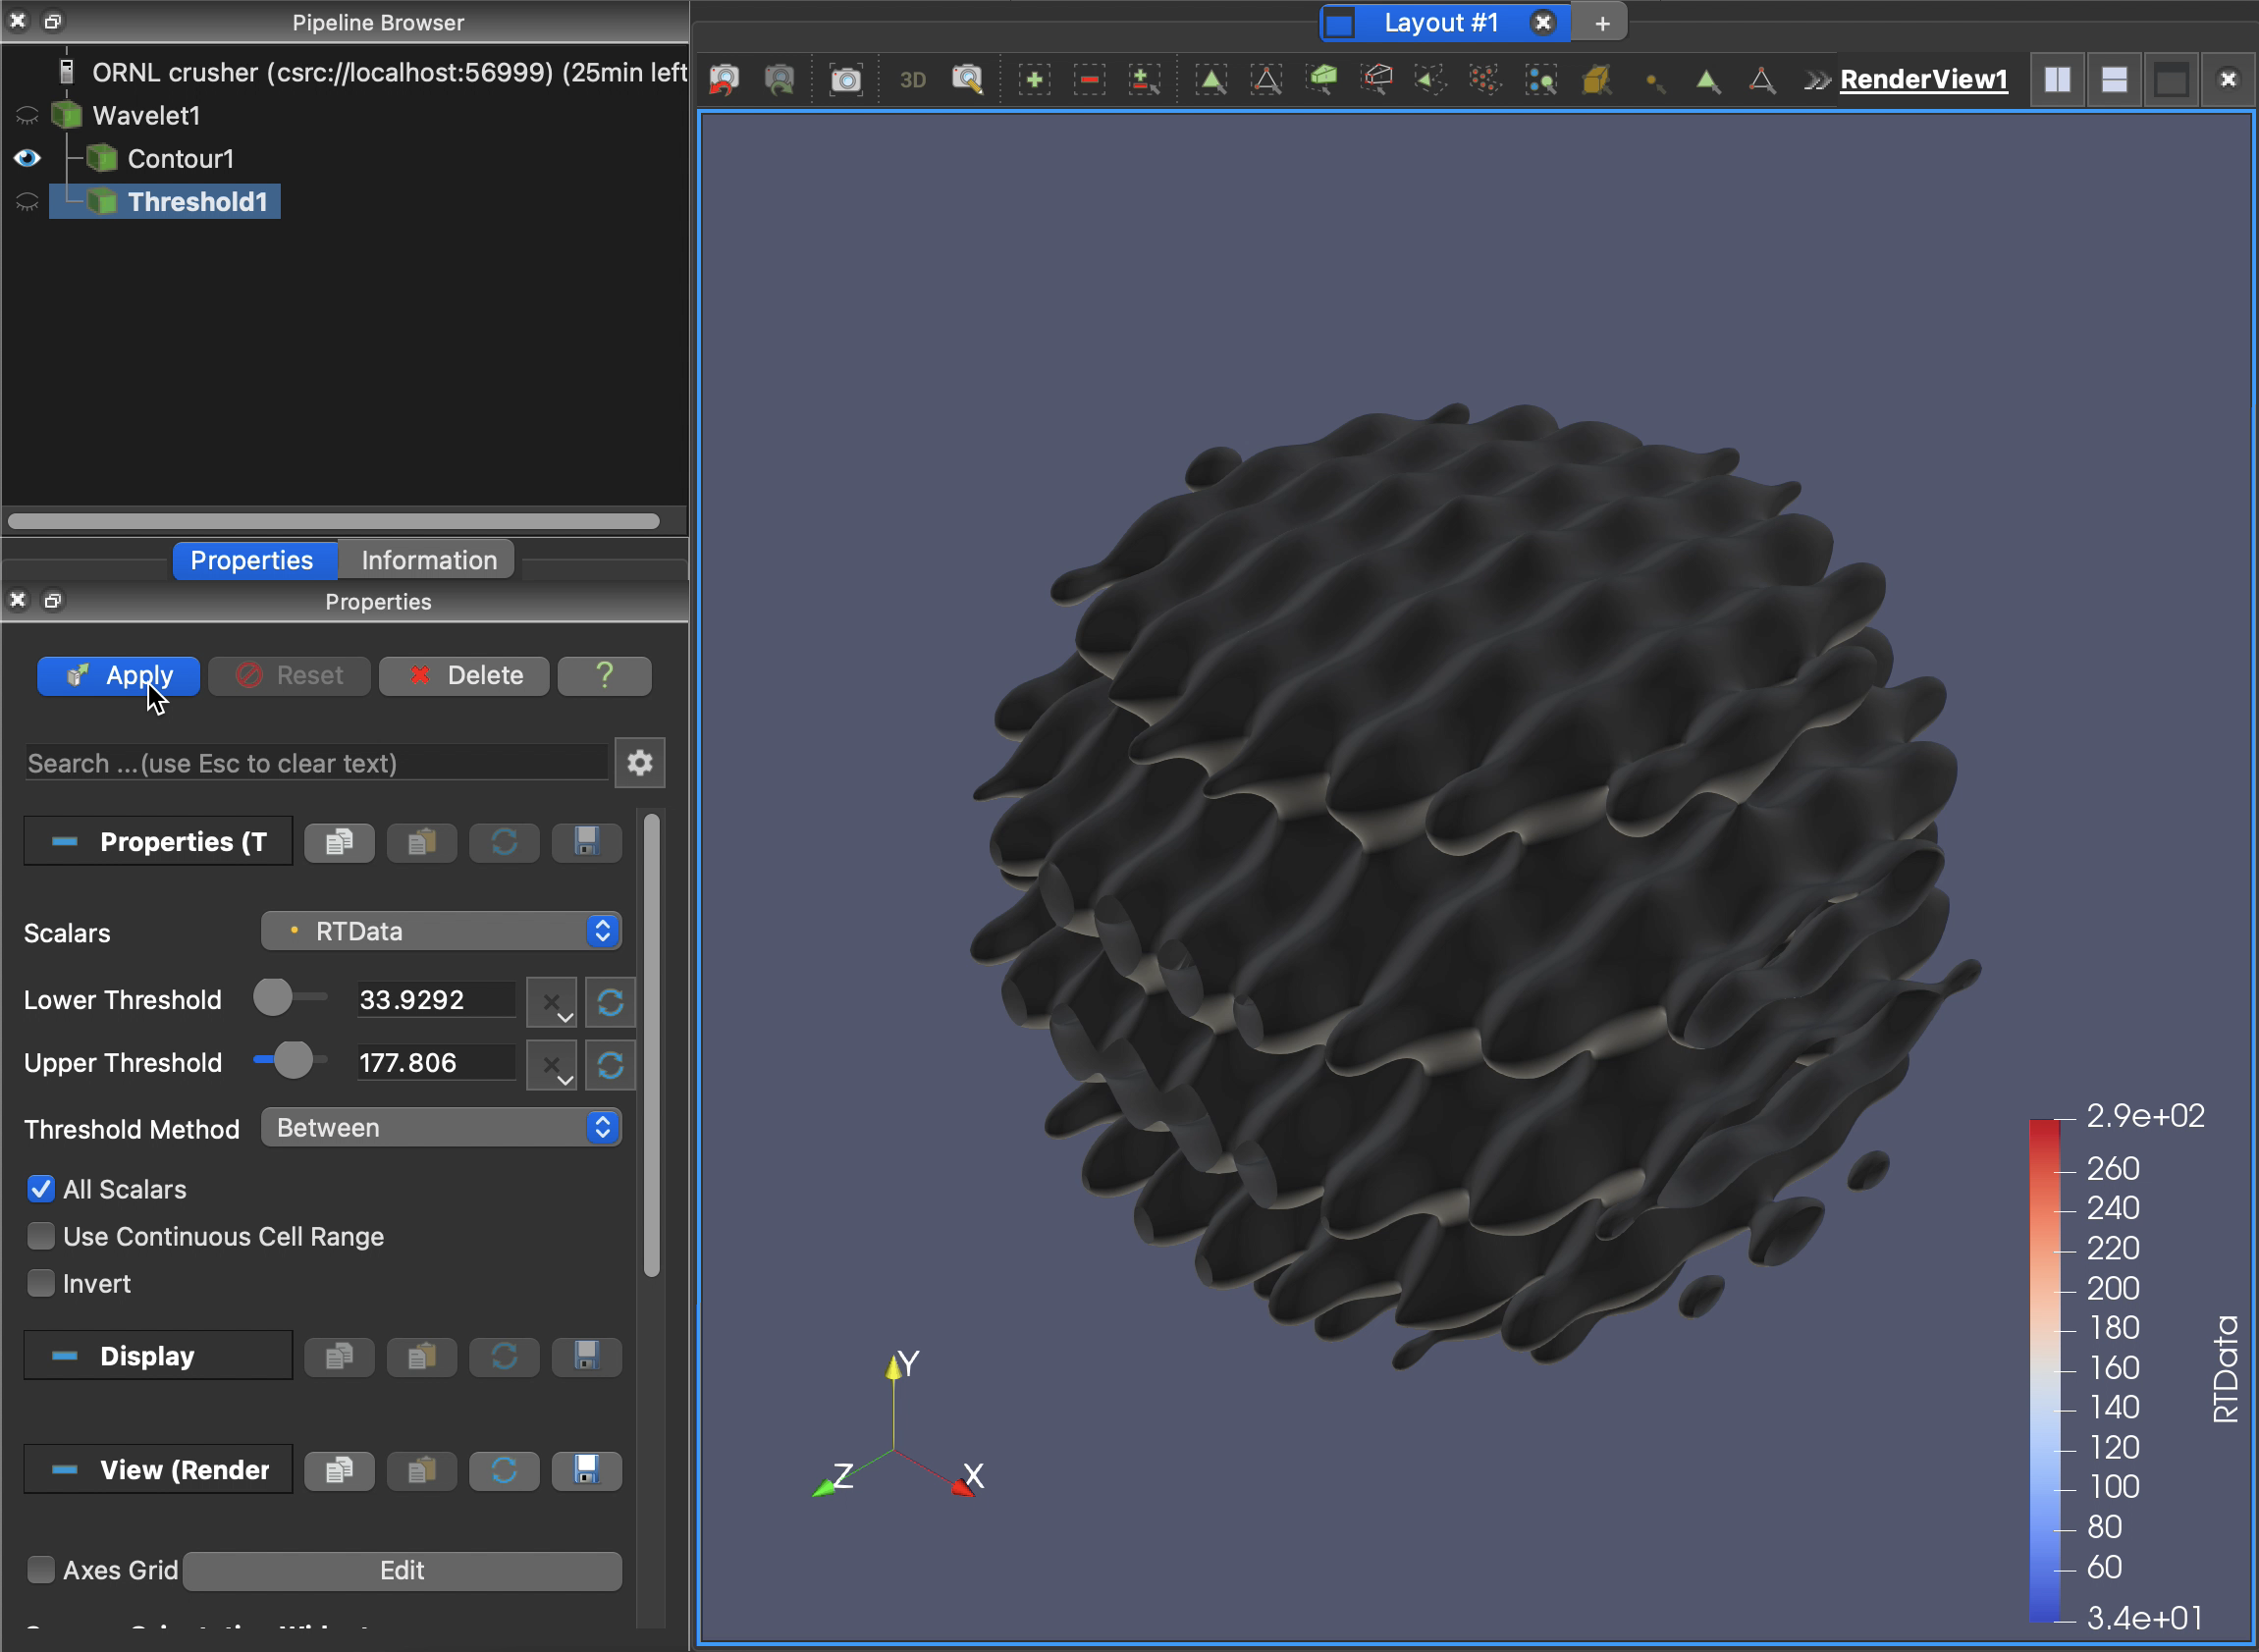
\includegraphics[width=\linewidth]{figures/paraview-crusher.png}
  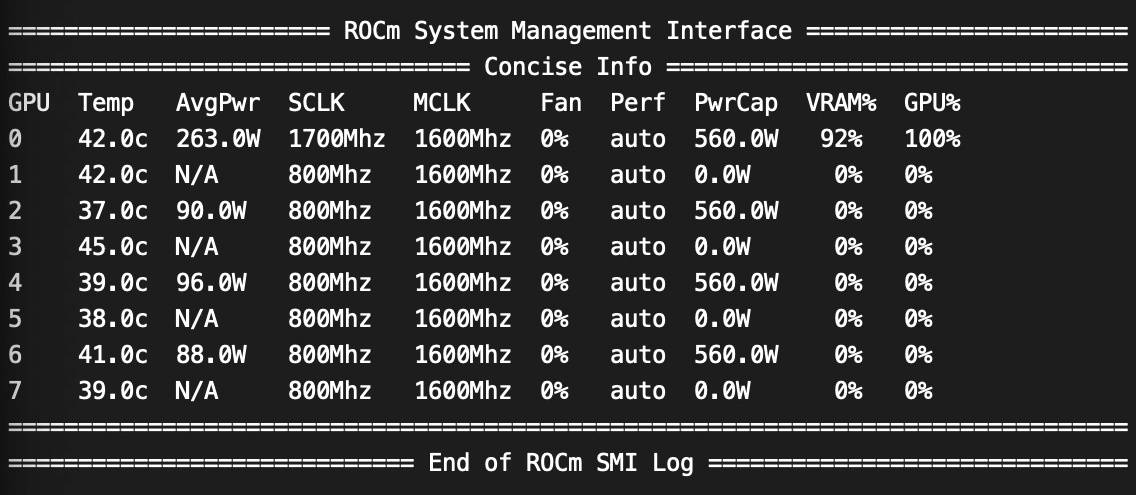
\includegraphics[width=\linewidth]{figures/threshold-vtkm-gpu-usage-crusher-small.png}
  \caption{ParaView, with integrated VTK-m accelerated filters, running on Crusher. VTK-m is using the Kokkos device adapter. The output of rocm-smi command is being used to verify and monitor GPU usage by the filters.}
  \label{fig:paraview-crusher}
\end{figure}

\sujin{
The first two paragraphs can be simplified by referring to the device adapter explanation in the VTK-m overview section
}
One of the main features that VTK-m supports is ‘write once, compile anywhere’ for its filters. VTK-m filter’s are implemented in modern C++. The build system of VTK-m can then compile these for one or more of the various parallel devices that it supports. This level of compatibility is achieved through the use of an abstraction layer in VTK-m called the \texttt{DeviceAdapter}. 

\texttt{DeviceAdapters} wrap a parallel execution capable device, providing functionalities for parallel-task scheduling, memory management, and several commonly used parallel algorithms like sort, reduce, etc, through a common interface. These are implemented on top of the native libraries used to program these devices. At the most basic level, a device adapter only needs to provide support for memory management on the device, a way to execute an n-way, fine-grained, parallel task on the device, and atomic operations. There are generic implementations for all of the parallel algorithms like sort, reduce, scan, etc, but it is possible to override these with specialized implementations for best performance. The early versions of VTK-m had \texttt{DeviceAdapter} implementations for single threaded CPUs using standard C++, multithreaded CPUs using the threading building blocks library or OpenMP, and GPGPUs using CUDA.

When the architectures for the initial two major exascale machines, Aurora and Frontier, were announced, it was revealed that they will be using two completely new GPGPU architectures, with their own native libraries (SYCL and HIP). This would have required additional two new device adapter backends. Maintaining these backends together with the already existing backends was would require a lot of effort, especially for a project that is primarily concerned with implementing highly parallel visualization algorithms.

For these reasons, we looked towards another ECP project called Kokkos~\cite{Edwards2014, Trott2022}. Kokkos is a library for implementing performance portable applications in C++. Similar to VTK-m, Kokkos also supports multiple device backends, including HIP and Sycl used by the exascale systems. So, with just one device adapter built on top of Kokkos, we are able to target both the machines.


\subsection{Removal of Virtual Methods}

\assign{Ken}

Ideally, an algorithm
%that operates on arrays
will know the data types that it will operate on.
Unfortunately, this is seldom the case for VTK-m where data ingested from different sources can have any number of basic types
%(32- or 64-bit floats or fixed precision values encoded in integers)
and different types of memory layout.
In the early years of ECP, this problem was addressed by compiling algorithms in VTK-m for all possible types that could be encountered.
However, the amount of potential cases generated is too large to be practical.
C++ objects with virtual methods are a natural solution to this problem, and as they became available on CUDA devices, VTK-m started using virtual methods to hide the structure of arrays.
However, this solution worked poorly and was later abandoned for two reasons.
First, using virtual methods introduced problems with library linking as the compilers had to collect any possible code that might be needed to be loaded on the device.
Second, when ECP announced that its Exascale machines would be using GPUs other than CUDA, it was unclear how well they would support virtual methods or even if they would be supported at all.

Consequently, the VTK-m development team pivoted.
Virtual methods were removed from the VTK-m code that ran on devices.
To manage the operations on types without using virtual methods, VTK-m employed a trio of strategies: multiplexing the type in the algorithm, generalizing the stride in arrays, and providing fallbacks when unexpected types were encountered.

The first strategy, multiplexing, required the use of a type agnostic storage object.
For this, a \texttt{Variant} class was added to VTK-m.
The \texttt{Variant} takes a list of types as template parameters, and it can hold exactly one of these objects at a time.
At runtime, the proper type can be queried and extracted.
%Implementing the \texttt{Variant} to avoid type punning across all device compilers was challenging.
Although multiplexing from a variant object still requires separate compilation for all possible types, it limits the code that must be recompiled to make it more manageable.

The second strategy required a redesign of the array management in VTK-m.
Where the original design of array management completely abstracted the implementation, the new design based array management on known buffers of memory.
This in turn provided a way to generalize the representation of an array component by defining a stride in the buffer.
In this way, an algorithm no longer had to be compiled for a specific data layout.
It could instead apply a stride to the array and use any layout.

The third strategy recognized that although a great number of types are possible, many are rarely if ever encountered in practice.
Therefore, instead of attempting to compile a function for any possible type, it is possible to instead compile for the most likely types and then have a fallback for the cases when the type is unexpected.
The typical solution is to copy the array of unknown type to an array of a known type.
This feature was included into the filter interface overhaul, which is described in the next section.

\subsection{Filter Interface Overhaul}

\assign{Ollie}

The addition of abstractions like `Variant` in VTK-m also allowed us to redesign the developer's interface for \texttt{Filters}. The original \textit{Filter} class used a rather complicated technique call \emph{Couriously recurring template pattern (CRTP)} emulate runtime polymorphism that is familiar to common object oriented programmers. Many other C++ template techniques were also used to match generic code in several \textit{}

\subsection{GPU-to-GPU Transfers}

Modern HPC GPUs allow direct GPU-to-GPU communication. This provides GPUs with an efficient mechanism to directly send data stored in their device memory to the target GPU device memory. This contrasts with the traditional and costly GPU communication pattern which consists in first copying the desired data from the device memory to host memory, transferring it, and then again copying the received data from host memory to device memory.

Enabling this feature in VTK-m required changes in the source code of both \begin{enumerate*} [label=\itshape(\alph*\upshape)]\item VTK-m and \item DIY\end{enumerate*}. The reason for making changes to DIY is that VTK-m delegates data marshaling and remote communication through the DIY library.

\textit{(a)} DIY library source code changes consisted in adding routines that allow sending and receiving raw pointers directly encapsulated in a newly introduced Blob data type. This contrasts with the regular operation of DIY that copies and serializes data before sending and receiving. In addition to that, we have also introduced a new API in DIY which controls the ownership of the passed raw pointer.

\textit{(b)} VTK-m source code changes consisted in changes to the VTK-m Buffer class and  adding a new CMake option named \texttt{VTKm\_ENABLE\_GPU\_MPI} which activates direct GPU-to-GPU communication of VTK-m Buffer objects. This in turn, enables direct GPU communication in VTK-m since most of the VTK-m storage entities are composed of VTK-m Buffers. 

The main challenge found during the implementation of this feature was maintaining compatibility with the target systems, OLCF Frontier. The challenged consisted in the fact that the software stack in the target system was a moving target with frequent updates that in many cases required us to tune build and runtime parameters and, in some other cases, perform changes to the VTK-m and DIY source code. This challenge was minimized by provisioning the VTK-m Gitlab project with nightly jobs that build and run tests that use this feature in the OLCF Frontier test-bed system (OLCF Crusher). 
